%\begin{savequote}[10cm]
%{\it ``The Three Laws of Robotics: \\
%1: A robot may not injure a human being or, through inaction, allow a human being to come to harm; \\
%2: A robot must obey the orders given it by human beings except where such orders would conflict with the First Law;\\
%3: A robot must protect its own existence as long as such protection does not conflict with the First or Second Law.''}
%\qauthor{Isaac Asimov}
%\end{savequote}

\chapter{Introduction} 
\label{Chap:Introduction}

This thesis was made with the spirit of contributing to the autonomy of humanoid robots; more precisely in the development of behaviors based on vision. Even with the tremendous expansion of humanoid robotics in the last years, the link between perception and motion generation is still not well developed. Hundreds of works covers both fields separately. In the perception side, vision is up today the main technique in humanoid robotics. 

There is an increasing interest in the development of humanoid robotics. Goverments and companies such as Honda, Boston Dynamics and Aldebaran Robotics have spent a lot of money in this fields. As result, it has been amazing demostrations in humanoid motions generation. However, generally the interaction with the environment is limited.

In Fig.~\ref{Fig:GeneralDiagram} we depict a general diagram of the workflow in humanoids. Generally we use computer vision to extract information from the environment (Mapping, localization, modeling). With this model we can plan the motion using rules given by a congnitive process. With this plan, the robot performs the dynamic walking which leads to the whole body motion. Generally computer vision requires high computational load to extract high level information from the scene; motion generation in the other side, requieres fast control loops to be dynamically stable. 

\begin{figure}[h]
\centering
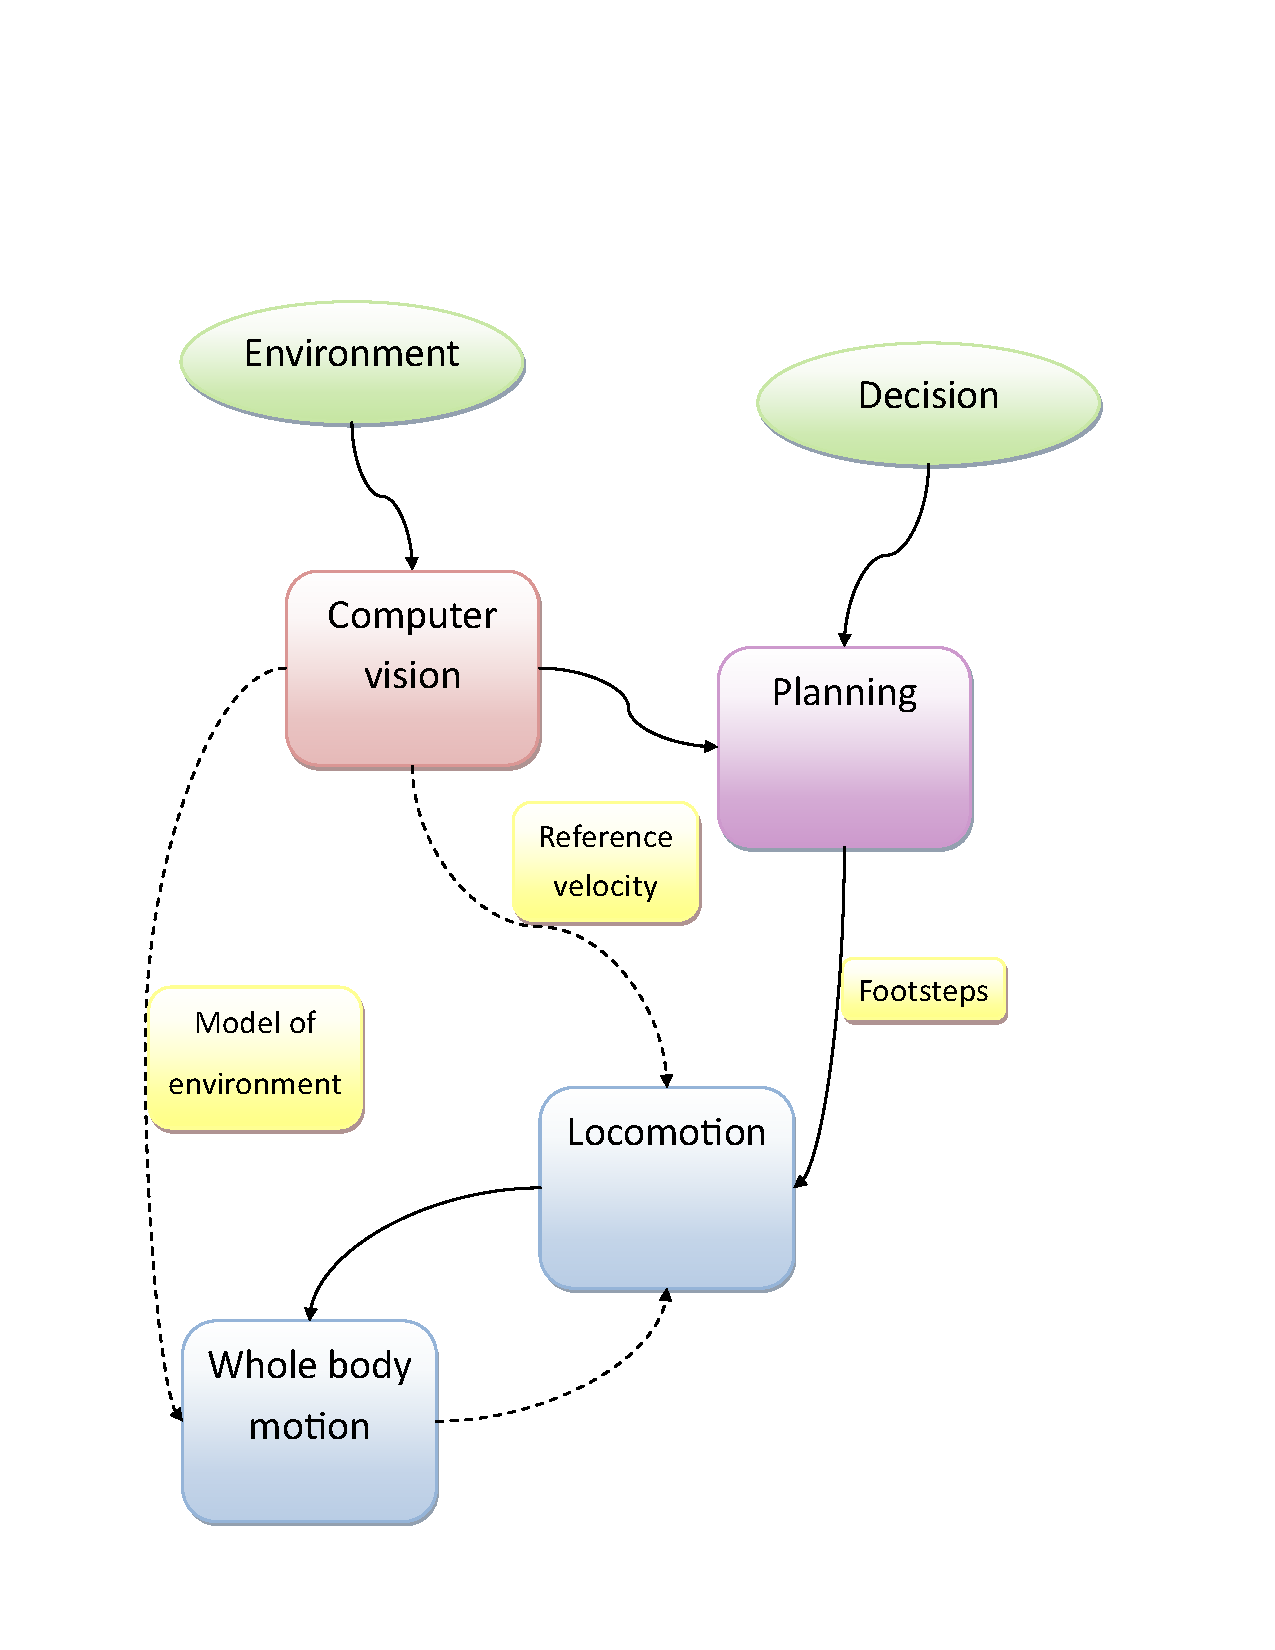
\includegraphics[scale=0.5]{figures/general-diagram.pdf}
\caption[]{ \label{Fig:GeneralDiagram} Workflow of a humanoid robot executing motion tasks using perception.}
\end{figure}

In this thesis we address the problem of the link between vision and motion generation. Building upon the work of several authors throw the years, our main contributions are,

\begin{itemize}
\item The fully integration of a visual servoing scheme within the walking motion generation using Linear Model Predictive Control (MPC);
\item The filling of the gap between traditional motion planning approaches and on-line locomotion generation algorithms;
\item The providing of 3D models of the escene in front of the robot to be used by an inverse-dynamics based approach to walk on rough terrain;
\item And finally, the validation in simulation of the proposals.
\end{itemize}

The rest of this manuscript is organized as follows. In chapter \ref{Chap:Related-Work} we state the problem and briefly recall the work that has been done on it. In chapter \ref{Chap:Visual-Servoing} We present an approach to introduce visual information in the walking pattern generator for humanoid robots. We make use of visual servoing withmodel predictive control (MPC), which is joined to the walking motion generator. Since visual servoing with MPC is a nonlinear optimization problem, we propose a linearization scheme in order to keep it as a Quadratic Program (QP) and introduce it within the pattern generator. In chapter \ref{Chap:Visual-Planning} we propose a method for reactive walking allowing visual servoing and adaptation of footsteps trajectories in real-time. This is done by building upon recent advances in the fields of optimal control for a walking pattern generator~\citep{HerdtAR2010} and planning for a nonholomic robot with field-of-view constraints ~\citep{Salaris:2010}. In chapter \ref{Chap:3DReconstruction} we present a 3D reconstruction system of the ground in front of the robot. This model allows to an inverse dynamics control scheme to know the ground structure where the swinging foot is going to step on. Finally in chapter \ref{Chap:Conclusions} we present the final discusion and future work.


